\chapter{TRIAC}
  \begin{wrapfigure}{R}{0.3\textwidth}
  \vspace{-1cm}
    \centering
    \resizebox{!}{\linewidth}{
    \begin{tikzpicture}
	\begin{pgfonlayer}{nodelayer}
		\node [style=none] (0) at (-1.5, 1.5) {};
		\node [style=none] (2) at (-1.5, 0.5) {};
		\node [style=none] (3) at (1.5, 0.5) {};
		\node [style=none] (4) at (-1.5, -0.5) {};
		\node [style=none] (5) at (1.5, -0.5) {};
		\node [style=none] (28) at (0, 1) {p};
		\node [style=none] (29) at (0, 0) {n};
		\node [style=none] (30) at (0, -1) {p};
		\node [style=none] (32) at (-0.5, 2.5) {};
		\node [style=none] (33) at (-0.5, 1.5) {};
		\node [style=none] (34) at (-1.5, 2.5) {};
		\node [style=none] (35) at (1.5, 0.5) {};
		\node [style=none] (37) at (0.5, -2.5) {};
		\node [style=none] (38) at (0.5, -1.5) {};
		\node [style=none] (39) at (1.5, -2.5) {};
		\node [style=none] (40) at (1.5, -1.5) {};
		\node [style=none] (41) at (-1, 2) {n};
		\node [style=none] (42) at (1, -2) {n};
		\node [style=none] (43) at (-1, 2.5) {};
		\node [style=none] (44) at (-1, 2.75) {};
		\node [style=none] (45) at (0, 2.75) {};
		\node [style=none] (46) at (0, 2.5) {};
		\node [style=none] (47) at (-1, -2.5) {};
		\node [style=none] (48) at (0, -2.5) {};
		\node [style=none] (49) at (-1, -2.75) {};
		\node [style=none] (50) at (0, -2.75) {};
		\node [style=none] (51) at (-0.5, 2.75) {};
		\node [style=none] (52) at (-0.5, 3.25) {};
		\node [style=none] (53) at (-0.5, 3.75) {$A_1$};
		\node [style=none] (54) at (-0.5, -2.75) {};
		\node [style=none] (55) at (-0.5, -3.25) {};
		\node [style=none] (56) at (-0.5, -3.75) {$A_2$};
		\node [style=none] (57) at (0.5, 1.5) {};
		\node [style=none] (58) at (0.5, 2.5) {};
		\node [style=none] (59) at (1.5, 2.5) {};
		\node [style=none] (60) at (1.5, 1.5) {};
		\node [style=none] (61) at (-1.5, -1.5) {};
		\node [style=none] (62) at (-0.5, -1.5) {};
		\node [style=none] (63) at (-0.5, -2.5) {};
		\node [style=none] (64) at (-1.5, -2.5) {};
		\node [style=none] (65) at (-1, -2) {n};
		\node [style=none] (66) at (1, 2) {n};
		\node [style=none] (67) at (0.75, 2.5) {};
		\node [style=none] (68) at (1.25, 2.5) {};
		\node [style=none] (69) at (1.25, 2.75) {};
		\node [style=none] (70) at (0.75, 2.75) {};
		\node [style=none] (71) at (0.75, -2.5) {};
		\node [style=none] (72) at (1.25, -2.5) {};
		\node [style=none] (73) at (1.25, -2.75) {};
		\node [style=none] (74) at (0.75, -2.75) {};
		\node [style=none] (75) at (1, -2.75) {};
		\node [style=none] (76) at (1, 2.75) {};
		\node [style=none] (77) at (1, 3.25) {};
		\node [style=none] (78) at (2.25, 3.25) {};
		\node [style=none] (79) at (2.25, 0) {};
		\node [style=none] (80) at (1, -3.25) {};
		\node [style=none] (81) at (2.25, -3.25) {};
		\node [style=none] (82) at (2.75, 0) {};
		\node [style=none] (83) at (3.25, 0) {G};
	\end{pgfonlayer}
	\begin{pgfonlayer}{edgelayer}
		\draw [style=fill2] (3.center) to (2.center);
		\draw [style=fill2] (2.center) to (35.center);
		\draw [style=fill2] (32.center) to (33.center);
		\draw [style=fill2] (33.center) to (0.center);
		\draw [style=fill2] (0.center)
			 to (33.center)
			 to (32.center)
			 to (58.center)
			 to (57.center)
			 to (60.center)
			 to (35.center)
			 to (2.center)
			 to cycle;
		\draw [style=fill2] (5.center) to (4.center);
		\draw [style=fill3] (4.center)
			 to (5.center)
			 to (3.center)
			 to (2.center)
			 to cycle;
		\draw [style=fill2] (37.center) to (38.center);
		\draw [style=fill2] (38.center) to (40.center);
		\draw [style=fill2] (5.center)
			 to (4.center)
			 to (61.center)
			 to (62.center)
			 to (63.center)
			 to (37.center)
			 to (38.center)
			 to (40.center)
			 to cycle;
		\draw [style=fill2] (5.center) to (4.center);
		\draw [style=fill3] (33.center)
			 to (32.center)
			 to (34.center)
			 to (0.center)
			 to cycle;
		\draw [style=fill3] (37.center)
			 to (39.center)
			 to (40.center)
			 to (38.center)
			 to cycle;
		\draw [style=fill4] (44.center)
			 to (45.center)
			 to (46.center)
			 to (43.center)
			 to cycle;
		\draw [style=fill4] (49.center)
			 to (50.center)
			 to (48.center)
			 to (47.center)
			 to cycle;
		\draw (51.center) to (52.center);
		\draw (54.center) to (55.center);
		\draw [style=fill3] (59.center)
			 to (60.center)
			 to (57.center)
			 to (58.center)
			 to cycle;
		\draw [style=fill3] (62.center)
			 to (61.center)
			 to (64.center)
			 to (63.center)
			 to cycle;
		\draw [style=fill4] (70.center)
			 to (67.center)
			 to (68.center)
			 to (69.center)
			 to cycle;
		\draw [style=fill4] (74.center)
			 to (73.center)
			 to (72.center)
			 to (71.center)
			 to cycle;
		\draw (76.center) to (77.center);
		\draw (77.center) to (78.center);
		\draw (78.center) to (79.center);
		\draw (79.center) to (82.center);
		\draw (81.center) to (79.center);
		\draw (81.center) to (80.center);
		\draw (80.center) to (75.center);
	\end{pgfonlayer}
\end{tikzpicture}

    }
    \caption{estructura interna del TRIAC.\protect\footnotemark}
    \label{fig:triac_si}
  \end{wrapfigure}
  \footnotetext{La region N de $A_1$ y $A_2$ es considerablemente mas grande que la de G en el dispositivo real. La figura es puramente ilustrativa.}
  Un triac es como un diac con una terminal compuerta. Un triac puede ser disparado por un pulso de corriente en la
  compuerta y no requiere voltaje de ruptura para iniciar la conducción, como el diac. Básicamente, se puede pensar en
  un triac simplemente como dos SCR conectados en paralelo y en direcciones opuestas con una terminal común, la
  compuerta. A diferencia del SCR, el triac puede conducir corriente en una u otra dirección cuando es activado, según
  la polaridad del voltaje a través de sus terminales A1 y A2. La figura \ref{fig:triac_si} muestra la construcción
  básica de un triac.

  \section{Curva característica del TRIAC}
    Para esta actividad de laboratorio, se propuso variar la tension de alimentacion en pasos grandes, variando entre
    cada paso la tension de gate $V_G$, observando el momento en el que se produzca el disparo del dispositivo. Ademas,
    se probara la capacidad del dispositivo de permanecer polarizado incluso cuando la tension de gate $V_G$ deja de
    estar presente. El circuito a implementar se puede ver en la figura \ref{crkt:triac_lab}.
    \begin{figure}[!ht]
      \centering
      \begin{minipage}{0.5\textwidth}
        \centering
        \begin{tikzpicture}
	% Paths, nodes and wires:
	\draw (3.25, -0.075) to[empty bidirectionaldiode] (6.25, -0.075);
	\draw (7.02, 1.5) to[empty triac, mirror] (7.02, -0.25);
	\draw (0.56, -0.075) to[qiprobe, l={$I_G$}] (3.25, -0.075);
	\draw (0, 0.925) to[american potentiometer, l={$R_V$}] (0, -1.075);
	\draw (7.02, 1.5) to[american resistor, l={$R_1$}] (7.02, 3.625);
	\draw (7.02, -0.25) to[qiprobe, l={$I_A$}] (7.02, -2.25);
	\draw (3.25, -0.075) to[qvprobe, l={$V_G$}] (3.25, -2.25);
	\node[vcc] at (7.02, 3.625){};
	\draw (0, 0.925) |- (0.02, 3.625) -- (7.02, 3.625);
	\draw (9.02, 3.625) to[qvprobe, l={$V_i$}] (9.02, -2.25);
	\draw (7.02, 3.625) -- (9.02, 3.625);
	\draw (9.02, -2.25) -| (0, -1.075);
\end{tikzpicture}
        \caption{circuito TRIAC a implementar en el laboratorio.}
        \label{crkt:triac_lab}
      \end{minipage}
      \hfill
      \begin{minipage}{0.4\textwidth}
        \centering
          \includegraphics[width=0.5\textwidth]{pictures/prot_triac.jpg}
        \caption{circuito TRIAC implementado en el laboratorio.}
      \end{minipage}
    \end{figure}

    \begin{table}[!ht]
      \centering
      \begin{tabular}{c|c|c|c|c|c|c|c|c}
        \multicolumn{3}{c|}{$V_i = 80V$} & \multicolumn{3}{c|}{$V_i = 130V$} & \multicolumn{3}{c}{$V_i = 180V$} \\
        $V_G \, [V]$ & $I_G \, [mA]$ & $I_A \, [mA]$ &  $V_G \, [V]$ & $I_G \, [mA]$ & $I_A \, [mA]$ & $V_G \, [V]$ & $I_G \, [mA]$ & $I_A \, [mA]$ \\ \hline
        0       & 0     & 0     & 0     & 0     & 0     & 0     & 0     & 0     \\
        10      & 0     & 0     & 10    & 0     & 0     & 10    & 0     & 0     \\
        20      & 0     & 0     & 20    & 0     & 0     & 20    & 0     & 0     \\
        30      & 0     & 0     & 30    & 0     & 0     & 30    & 0     & 0     \\
        31      & 0     & 0     & 31    & 0     & 0     & 32    & 0     & 31.7  \\
        32      & 3.4   & 3.4   & 31.6  & 4.53  & 4.57  &       &       &       \\
        23.3    & 3.8   & 3.9   & 28.4  & 4.53  & 4.53  &       &       &       \\
        23.1    & 4.15  & 4.15  & 0.3   & 0     & 26.7  &       &       &       \\
        23.2    & 4.6   & 4.8   &       &       &       &       &       &       \\
        23.2    & 4.3   & 6     &       &       &       &       &       &       \\
        23.3    & 4.1   & 6.2   &       &       &       &       &       &       \\
        0.7     & 0     & 16.3  &       &       &       &       &       &       \\
      \end{tabular}
      \caption{valores relevados en el laboratorio.}
      \label{tab:triac_curvcar_lab}
    \end{table}

\begin{figure}[!ht]
  \centering
  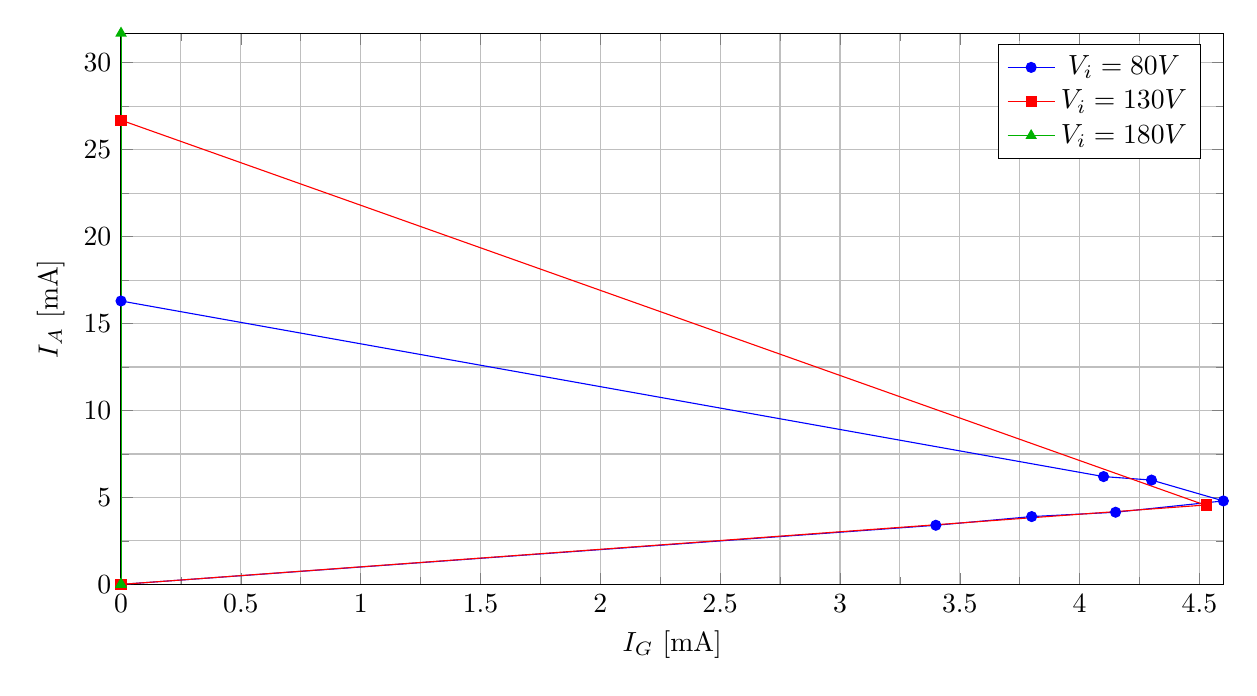
\begin{tikzpicture}
    \begin{axis}[
      width=14cm,
      height=7cm,
      xlabel={$I_G$ [mA]},
      ylabel={$I_A$ [mA]},
      grid=both,
      minor tick num=1,
      scale only axis,
      enlargelimits=false,
    ]

    % --- Datos para Vi = 80V ---
    \addplot[
      color=blue,
      mark=*,
      mark size=1.8pt
    ] coordinates {
      (0,0)
      (0,0)
      (0,0)
      (0,0)
      (0,0)
      (3.4,3.4)
      (3.8,3.9)
      (4.15,4.15)
      (4.6,4.8)
      (4.3,6)
      (4.1,6.2)
      (0,16.3)
    };
    \addlegendentry{$V_i = 80V$}

    % --- Datos para Vi = 130V ---
    \addplot[
      color=red,
      mark=square*,
      mark size=1.8pt
    ] coordinates {
      (0,0)
      (0,0)
      (0,0)
      (0,0)
      (0,0)
      (4.53,4.57)
      (4.53,4.53)
      (0,26.7)
    };
    \addlegendentry{$V_i = 130V$}

    % --- Datos para Vi = 180V ---
    \addplot[
      color=green!70!black,
      mark=triangle*,
      mark size=2pt
    ] coordinates {
      (0,0)
      (0,0)
      (0,0)
      (0,0)
      (0,0)
      (0,31.7)
    };
    \addlegendentry{$V_i = 180V$}

    \end{axis}
  \end{tikzpicture}
  \caption{Familia de curvas experimentales $I_A = f(I_G)$ para distintos valores de $V_i$}
  \label{graph:triac_curvcar_lab}
\end{figure}
  \section{Recortador de onda con TRIAC}
